\section{Problem 1}\label{problem1}
The KKT conditions for this problem is as follows: 

\begin{equation}
    A^T\lambda^*+s^*=c
\end{equation}

\begin{equation}
    Ax^*=b
\end{equation}

\begin{equation}
    x^*\geq0
\end{equation}

\begin{equation}
    s^*\geq0
\end{equation}

\begin{equation}
    s^*_ix^*_i=0, \space i = 1,...,n
\end{equation}

\subsection{a} \label{1a}
 

\includegraphics[width=1\linewidth]{Figures/1a.png}

\subsection{b} \label{1b}

From the book we have:

    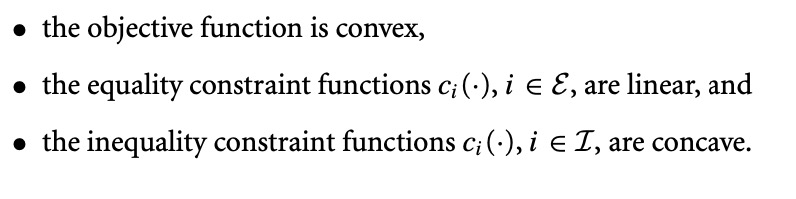
\includegraphics[width=\linewidth]{Figures/1b_book.jpeg}

And we also have the formal definition of a convex function:

    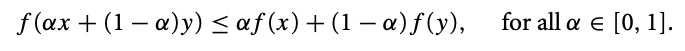
\includegraphics[width=\linewidth]{Figures/1bdef.jpeg}



